\documentclass[tikz,border=15pt]{standalone}
\usepackage{amsmath}
\usetikzlibrary{positioning, arrows.meta}

\begin{document}
	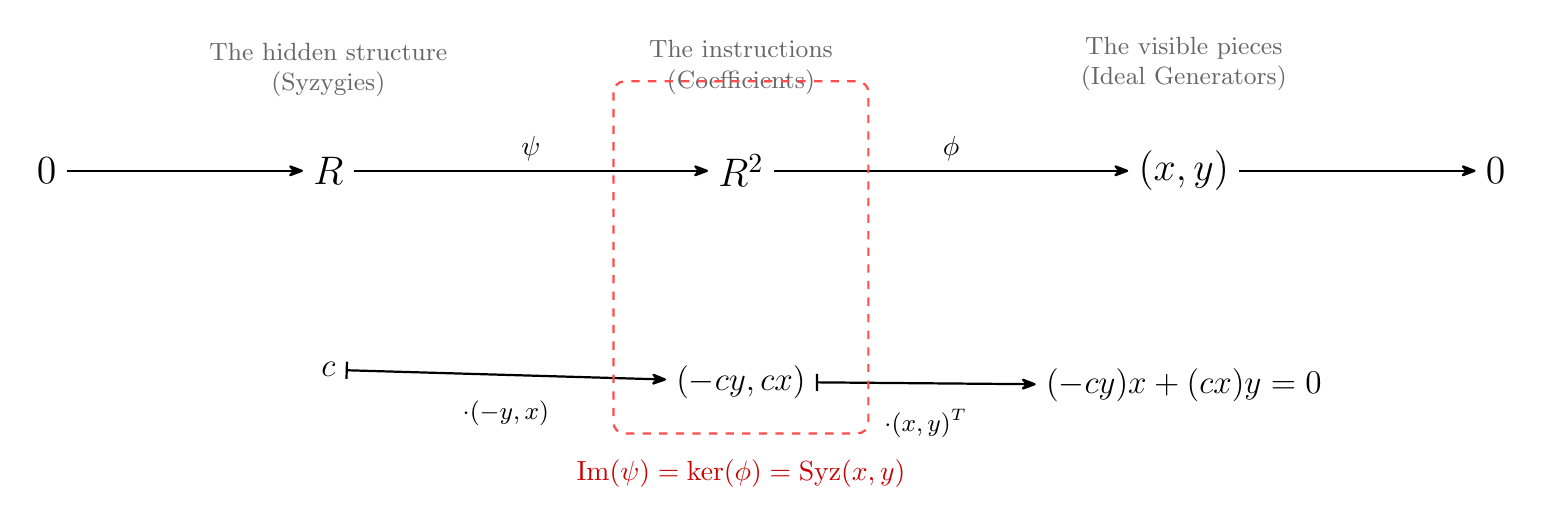
\begin{tikzpicture}[
		node distance=3cm,
		auto,
		module/.style={font=\Large\bfseries},
		element/.style={font=\large},
		annotation/.style={font=\small\color{gray!80!black}, align=center},
		->, >={Stealth[round]}, thick
		]
		
		% --- Module Level (Exact Sequence) ---
		\node[module] (0_left) {$0$};
		\node[module] (R) [right=of 0_left] {$R$};
		\node[module] (R2) [right=of R, xshift=1.5cm] {$R^2$};
		\node[module] (I) [right=of R2, xshift=1.5cm] {$(x,y)$};
		\node[module] (0_right) [right=of I] {$0$};
		
		% Module Maps
		\draw (0_left) -- (R);
		\draw (R) -- node[above] {$\psi$} (R2);
		\draw (R2) -- node[above] {$\phi$} (I);
		\draw (I) -- (0_right);
		
		% Conceptual Annotations above the modules
		\node[annotation, above=0.5cm of R] {The hidden structure\\(Syzygies)};
		\node[annotation, above=0.5cm of R2] {The instructions\\(Coefficients)};
		\node[annotation, above=0.5cm of I] {The visible pieces\\(Ideal Generators)};
		
		% --- Element Level ---
		\node[element] (c) [below=2cm of R] {$c$};
		\node[element] (pair) [below=2cm of R2] {$(-cy, cx)$};
		\node[element] (zero) [below=2cm of I] {$(-cy)x + (cx)y = 0$};
		
		% Element Maps (mapsto)
		\draw[|->] (c) -- node[below=0.2cm, font=\small] {$\cdot (-y,x)$} (pair);
		\draw[|->] (pair) -- node[below=0.2cm, font=\small] {$\cdot (x,y)^T$} (zero);
		
		% --- Kernel Highlight ---
		% A subtle red dashed box to frame the syzygy module's placement in R^2
		\draw[dashed, -, red!70, rounded corners]
		([xshift=-1.2cm, yshift=0.8cm]R2.north west) rectangle ([xshift=1.2cm, yshift=-3cm]R2.south east);
		\node[red!80!black, align=center, font=\normalsize, below=3.2cm of R2] {$\operatorname{Im}(\psi) = \ker(\phi) = \operatorname{Syz}(x,y)$};
		
	\end{tikzpicture}
\end{document}